\chapter{Implementation Analysis}
\label{chap:analysis}

Just like other modern day circuit simulators, our library is also heavily influenced by the original Berkeley SPICE. We have decided to reflect this fact in the name our library and call it NextGen SPICE, and we will use this name in the remainder of this thesis.

This chapter analyses various possibilities of NextGen SPICE simulator implementation. The reader should be acquainted with the necessary theory of circuit simulation. Ron Kielkowski's Inside SPICE \cite{inside_spice} is an excellent source of details about the workings of SPICE-like simulators. The necessary mathematical theory is nicely summarized in the documentation of the QUCS simulator \cite{qucs}, which we will cite frequently in the next chapters. Another great source is the Ph.D. theses of Laurence W. Nagel (Author of SPICE2) \cite{Nagel:M520}. The last two sources are freely available and we include them on the attached CD for convenience.

\section{Initial Organisation of the library}

One of the goals of this thesis is the implementation of a configurable and extensible circuit simulation library. One of the requirements is that new types of circuit analyses as well as new circuit devices can be added without modification of the core library's source code (goal~\ref{goal:extension}). Before we start with the actual analysis, we will briefly describe how the original SPICE program operates. 

\subsection{Overview of SPICE Simulator Workflow}
\label{chap:analysis:spice-review}
The top level view on the SPICE simulator is summarized in figure~\ref{fig:spice-workflow}. The user specifies the circuit to be simulated inside a SPICE netlist file (1). This file is parsed by SPICE, which constructs an internal representation of the circuit (2) and validates the circuit topology according to the rules described in section~\ref{chap:spicecode:topology}. If the circuit is correctly formed, SPICE performs the simulations specified in the netlist file. This consists of mapping the devices into coefficients in an equation system characterizing the circuit (3). This equation system is then solved to obtain the result of the analysis, which is then stored in the circuit representation. The user-specified characteristics of the circuit devices are then printed to the output (4). 

\begin{figure}[h]
	\centering
	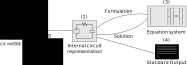
\includegraphics[width=0.8\linewidth]{spice-workflow}
	\caption{SPICE operation workflow.}
	\label{fig:spice-workflow}
\end{figure}


Because different analyses simulate different characteristics of circuit devices, most devices contribute to the equation system coefficients differently in each circuit analysis. To provide a concrete example, the following two paragraphs briefly describe two distinct kinds of circuit analyses: transient analysis (the implementation of which is part of this thesis), and AC frequency sweep analysis (which we would like to implement in future versions), and their specific way of simulating capacitors and inductors.

In transient analysis, the circuit's behavior is simulated over time. The first step of this analysis is calculating the initial DC bias of the circuit, which is the technical term for calculating the node voltages and currents flowing through the circuit branches. During this step, capacitors are modeled as ideal open circuits and inductors as ideal short circuits.\footnote{Consequence of modeling capacitor as open circuit and inductor as short circuit is that the simulation starts from a stable (quiescent) state of the circuit, SPICE simulators allow user to specify custom initial conditions: voltage across the capacitor and current flowing through the inductor, and thereby starting the simulation from an unstable state.} In subsequent timepoint calculations, capacitor and inductor devices are modeled by equivalent subcircuits consisting of a voltage or current source and a resistor. Values of voltage, current and resistance in these equivalent subcircuits are recomputed at each timepoint to reflect the energy storing behavior of these devices.

AC frequency sweep analysis simulates how a circuit behaves when a signal of certain frequency is applied to it. As opposed to transient analysis, which iterates over time, AC frequency sweep iterates over frequencies of the applied signal. It also starts by calculating the DC bias of the circuit, but after that, nonlinear characteristics of circuit devices are not modeled. Instead the behavior of each device around the established DC operating point is considered to be linear, which simplifies the analysis. Contrary to transient analysis which models the energy storing behavior of capacitors and inductors, AC frequency sweep models their reactance, which depends on the signal frequency and the device's capacitance and inductance, respectively. An additional difference between transient and AC frequency sweep analyses is that in AC frequency sweep analysis, the equation system that characterizes the circuit contains complex numbers as coefficients, whereas in transient analysis, only real numbers are needed.\footnote{Additional details about how capacitors and inductors are modeled can be found in QUCS technical papers. For trasient analysis, see sections 6.3.1 and 6.3.2 for capacitor and inductor, respectively; and for AC analysis see sections 9.3 for capacitor and 9.4 for inductor. More detailed description of individual SPICE circuit analyses can be found in chapter 2 of Inside SPICE p. 37--41}

\subsection{Separating Circuit Analyses}
\label{chap:analysis:separation}
Suppose we used the same workflow as in figure~\ref{fig:spice-workflow} and implemented transient analysis via instance methods on the circuit representation. When we would want to implement AC frequency sweep analysis in the simulator, we would have to modify the circuit representation and add new methods and data fields, which contradicts our goal of extensibility (goal~\ref{goal:extension}). In order to leave the transient analysis implementation intact, we would have to create a brand new circuit representation that would implement the operations needed by AC frequency sweep analysis.

Having multiple implementations of the circuit representation may seem to be excessive code duplication. However, as we have described in the previous paragraphs, the implementation of AC frequency sweep analysis would be quite different from that of transient analysis: different contributions to the circuit equation system, usage of complex numbers in the equation system, and no need for updating the inner state of the device. Because the two types of analyses are conceptually different, implementing them separately could actually improve the readability and maintainability of the code base.

To allow performing different circuit analyses without having to create the specific circuit representation manually for each analysis, we decided to modify the workflow shown into the one shown in figure~\ref{fig:library-workflow}. We introduced an analysis-independent circuit description (which we will simply refer to as a \textit{circuit description}), which would be used to automatically create the analysis-specific circuit representation (which, we will refer to as a \textit{circut model} for brevity) on-demand. The library functionality can be thus partitioned into analysis-independent and analysis-dependent parts as illustrated in the figure.

\begin{figure}[h]
	\centering
	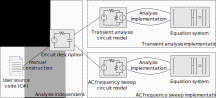
\includegraphics[width=\linewidth]{library-workflow}
	\caption{Workflow used in NextGen SPICE library}
	\label{fig:library-workflow}
\end{figure}

\subsection{Devices and Device Models}
\label{chap:analysis:device-models}
We have also stated that we would like the possibility of adding a new devices in the future. To achieve that, transient analysis (and each other analysis to be implemented) should specify operations required from each device via an interface. Adding new device would consist of implementing this interface for each analysis type. Figure~\ref{fig:analysis-interface} illustrates a possible device implementation hierarchy. Suppose that transient analysis requires the \texttt{ITransientDevice} interface, and AC frequecy sweep requires the \texttt{IAcFreqSweepDevice} interface. We have already described that capacitor and inductor devices are handled differently in both of these analyses, and it would make sense to implement the behavior separately for each analysis. At the same time, some devices -- such as resistors -- are handled the same way. The implementation of the resistor device could possibly implement both interfaces in the same class.

\begin{figure}[h]
	\centering
	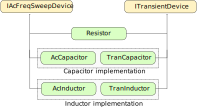
\includegraphics[width=0.7\linewidth]{analysis-interfaces}
	\caption{Implementation of devices for different circuit analyses}
	\label{fig:analysis-interface}
\end{figure}

Furthermore, we also stated in the requirements that it should be possible to easily change how each device is simulated. As an example, consider a BJT transistor device. During transient analysis, a BJT transistor can be modeled by using either the Ebers-Moll model or the more detailed Gummel-Poon model. Other analysis types can potentially use different transistor models. We would like to allow users to select which device model\footnote{To avoid possible confusion with \texttt{.MODEL} statements used in netlist files, this thesis uses term \textit{device model} exclusively to refer to the set of equations describing the device's behavior (such as the mentioned Ebers-Moll model). The entities described by \texttt{.MODEL} statement are referred to as \textit{device model parameters}.} should be used for the BJT device (and other devices as well). This will allow the library to be used for comparing existing device models and developing new ones. A concrete example hierarchy of the classes, which can be used to model a BJT transistor in transient and AC frequency sweep analyses, is illustrated in figure~\ref{fig:analysis-separation}. The classes \texttt{TranEbersMollBjt} and \texttt{TranGummelPoonBjt} implement the operations required by transient analysis for the respective transistor device models. During AC freqency sweep analysis, a completely different model (Hybrid-pi) is used, which is implemented by the \texttt{AcHybridPiBjt} class.

\begin{figure}[h]
	\centering
	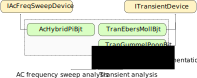
\includegraphics[width=.7\linewidth]{transient-separation}
	\caption{Separation of device implementation for each analysis type.}
	\label{fig:analysis-separation}
\end{figure}


\subsection{Splitting to Multiple Assemblies}
\label{chap:analysis:splitting}

A straightforward way of implementing the library would be putting everything into one assembly. However, that means that after each modification, the whole library has to be replaced by the new version. In the preceding section we decided to make the implementation of individual analysis types independent of each other, with a separate set of classes for representing the circuit under analysis. As developers, we would like to be able to develop, update and deploy each type of circuit analysis independently of the other types. In order to achieve that, we decided to organize the library into assemblies as illustrated in figure~\ref{fig:library-modules}. The \texttt{NextGenSpice.Core} is a shared assembly containing analysis-independent parts of the library, and is referenced by assemblies implementing individual analysis types. The implementation of the circuit model for transient analysis will be contained in the \texttt{NextGenSpice.LargeSignal} assembly. We chose the name LargeSignal because the resulting model allows transient, DC sweep and DC operating point analyses, which all rely on the large-signal model of circuit devices.

\begin{figure}[h]
	\centering
	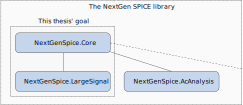
\includegraphics[width=0.8\linewidth]{analysis-modules}
	\caption{General organisation of the analysis types in the library.}
	\label{fig:library-modules}
\end{figure}

The \texttt{NextGenSpice.Core} assembly should have no knowledge of the assemblies containing the analysis types. To achieve that, we will make use of a principle called \textit{inversion of control} (IoC). In simple words, each assembly containing the implementation of a circuit analysis type should inform the \texttt{NextGenSpice.Core} assembly of its existence and instruct it how its circuit model can be created from the circuit description.

To make this procedure automatic without any action needed from the library's user, we decided to use an IoC framework. The functionality we require from the framework is quite simple and available in most IoC frameworks (importing implementations of certain interface from assemblies in the same directory as the core library). We decided to use the MEF framework \cite{mef} by Microsoft, which is distributed as a NuGet package and is standardly used. Another attractive feature of MEF is that it allows exporting classes by simply adding an \texttt{[Export]} attribute. 

In this section we described the reasons for the overall design of the NextGen SPICE library; in the sections that follow, the individual components of the library are analyzed in greater depth.

\section{NextGenSpice.Core}

The \texttt{NextGenSpice.Core} assembly will be the integral part of NextGen SPICE. It should contain the analysis-independent parts of the library: the circuit description classes, faculties for composing and validating the circuit, and the central mechanism that allows creation of analysis-specific circuit models. These parts will be discussed in the following subsections.

\subsection{Representation of the Circuit}
\label{fig:analysis:representation-circuit}
In the previous section we made the important decision to introduce separate sets of classes for circuit representation for each circuit analysis type. We have also decided to create another separate circuit description from which these analysis-specific representations should be constructed on-demand. The circuit description should be encapsulated in a single object of class \texttt{CircuitDefinition} for easy manipulation. The following subsubsections consider individual aspects of representing the circuit.

\subsubsection{Representing Circuit Nodes} 
In the SPICE netlist syntax, as described in chapter~\ref{chap:spicecode}, we allow circuit nodes to be identified by arbitrary alphanumeric strings, which would make the C\# type \texttt{string} a straightforward choice.

However, the main reason for using strings in the netlist syntax was probably to let users choose convenient names and make the netlists more readable. During the actual simulation and equation formulation, the circuit nodes need to be numbered in order to map the devices to corresponding equation matrix entries, and it would be more natural to use numbers to identify the circuit nodes. 

Because we do not expect users of the NextGen SPICE library to compose large circuits in the source-code manually, we decided to use the C\# type \texttt{int} for identifying individual nodes. This also implies that we need to translate circuit node names while parsing SPICE netlists into node indices, and provide this mapping to the user.

\subsubsection{Representing Individual Devices}
\label{chap:analysis:representation}
We need a circuit device representation which allows simple adding of new devices. A natural way of representing cicruit devices in an OOP language like C\# is introducing a class per circuit device, which all implement the same interface, e.g. \texttt{ICircuitDefinitionDevice}. This would lead to a hierarchy parallel to that of the analysis-specific device implementation classes from section~\ref{chap:analysis:device-models}. Having these multiple parallel hierarchies would simplify implementation of the analysis-specific circuit model creation, because all it would need is a mapping between these two hierarchies, as illustrated in figure~\ref{fig:03-fig-definition-hierarchy}.

\begin{figure}[h]
	\centering
	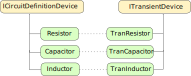
\includegraphics[width=0.57\linewidth]{definition-hierarchy}
	\caption{Mapping between circuit definition and analysis implementation classes}
	\label{fig:03-fig-definition-hierarchy}
\end{figure}


All data specific for any particular device would be stored in the respective properties of the device's class, and new devices can be added by creating another implementation of the \texttt{ICircuitDescriptionDevice} interface. Since this circuit device representation meets our requirements, we decided to use it.

\subsubsection{Representing subcircuits}
An important feature of SPICE netlists which we need to take into consideration when designing the circuit representation is the subcircuit feature (see section~\ref{chap:spicecode:subcircuits}).

Since a subcircuit can be used multiple times throughout a netlist file (i.e.\ multiple \texttt{X} statements with the same subcircuit name), we have decided to create separate classes \texttt{SubcircuitDefinition} for the description of the subcircuit  and \texttt{SubcircuitDevice} for the usage of the subcircuit. The subcircuit definition would need to store data about the inner devices and nodes, and which nodes are the connections to the outside circuit. The \texttt{SubcircuitDefinition} instances would be shared among potentially many \texttt{SubcircuitDevices}, which store data about the outside nodes to which the subcircuit is connected. 

%\todo{figure?}

\subsubsection{Enforcing Circuit Topology}
In section~\ref{chap:spicecode:topology}, we described circuit topology restrictions that we will impose on the circuit to ensure that the circuit equations during the simulation have a unique solution. Also, we want to prohibit the user from making changes to the circuit topology during the circuit simulation, because it could cause the circuit to be no longer valid. We would also like to diagnose any circuit topology violations as soon as possible, preferably immediately after the whole circuit is constructed.

Changes to the circuit topology could be achieved by two ways: adding or removing a whole device, and changing the nodes to which the device was connected. Both can be forbidden by making the circuit description read-only. However, that would mean that all circuit devices would have to be supplied at once to the \texttt{CircuitDefinition} constructor, and the validation would have to be performed inside the constructor.

To move the validation code outside the \texttt{CircuitDefinition} class, we will use a separate class \texttt{CircuitBuilder} to incrementally add new devices, and perform the validation before creating the actual \texttt{CircuitDefinition} class instance.

\subsection{Creating Analysis-specific Circuit Representations}
Back in section~\ref{chap:analysis:separation}, we decided to introduce multiple parallel hierarchies for representing the electrical circuit, each one for a particular circuit analysis. In order for the library to be easy to use, the user should not have to create these representations separately for each circuit analysis type manually. Instead, the library should provide a way to create the analysis-specific circuit representations automatically.

An ideal user interface of the library would allow the user to specify a mapping between the circuit description classes as discussed in section~\ref{chap:analysis:representation}. If the user then requested the transient analysis circuit representation, the library would then use this mapping to instantiate classes that implement the transient analysis logic for each device from the circuit description, and return the result back to the user.

This mapping will also be used to specify which device model should be used during the analysis. To allow simple comparing of different device models (such as the Ebers-Moll or Gummel-Poon BJT transistor models, which would each be implemented as a separate class, as discussed back in section~\ref{chap:analysis:device-models}), we would like to allow users to potentially specify multiple sets of mappings for a certain analysis type.

We have therefore decided to encapsulate these mappings in a \textit{factory class}. However, the concrete class type of the analysis-specific circuit representation is not known, because the \texttt{NextGenSpice.Core} assembly does not contain any analysis-specific functionality. We will therefore use a class hierarchy similar to the one in figure~\ref{fig:analysis-model-factories}. We will use the generic class feature of C\# and implement an abstract \texttt{AnalysisModelFactory<T>} class with one generic parameter for the circuit representation class type. This abstract class will implement methods for managing the mappings between a device description and implementation classes (symbolized by the \texttt{SetModel} method). The actual instantiation of the analysis-specific circuit model (\texttt{LargeSignalCircuitModel} on the figure) is delegated to derived classes, which provide a way to create new methods by implementing the abstract \texttt{NewInstance} method.

\begin{figure}[h]
	\centering
	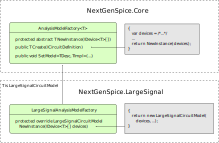
\includegraphics[width=0.9\linewidth]{analysis-factories}
	\caption{Relationship between analysis model factories}
	\label{fig:analysis-model-factories}
\end{figure}

In section~\ref{chap:analysis:splitting}, we decided to use the MEF framework to automatically discover the available analysis types. This means that each assembly with a circuit analysis implementation needs to export its own class derived from \texttt{AnalysisModel\+Factory<T>}. To provide a convenient place to aggregate the exported factories, we introduced yet another class: \texttt{AnalysisModelCreator}, which serves as a container for the analysis circuit model factories. The actual analysis model creation can be then implemented as a generic method on \texttt{AnalysisModelCreator}, which will then find the appropriate factory to be used for the construction of the desired circuit model class specified as the type argument.

\section{SPICE Netlist Parser}
\label{chap:analysis:parser}
An important feature of our library is to allow users to import subcircuits from SPICE netlist files (Goal~\ref{goal:parser}). Therefore, a SPICE netlist parser needs to be implmented.

Both the lexer and parser can be either written manually or be generated by a tool. In .NET ecosystem, possible choices include tool generators such as ANTLR \cite{antlr}. When using these generator tools, the language is described by a set of regular expressions and formal grammar rules, and the tool then generates the implementation of the lexer and parser.

Since the SPICE netlist grammar has a simple structure and a hand-written parser would be easy to write, we have come to the conclusion that the generator tools would only add unnecessary complexity to the library's implementation, and we will therefore implement the parser manually. 

\section[Double-double and Quad-double Arithmetic]{Double-double and Quad-double \\ Arithmetic}
\label{chap:analysis:dd}
According to goal~\ref{goal:dd} of this thesis, the library should allow representing real numbers with greater precision using the double-double and quad-double technique. The implementation of these techniques is very complex and requires deep knowledge and understanding of the algorithms to be done correctly. Therefore, we will not implement double-double and quad-double arithmetic ourselves, but we will use a third party library to provide that functionality.

During our search for a suitable library, we did not find any implementation of double-double or quad-double in .NET. However, we discovered a C++ implementation by Hida et al. called QD \cite{qd-lib} which is available under the BSD license. Even though our library will be targeted at .NET Standard, we still can use this library because .NET Standard version 2.0 requires implementations of .NET to provide PInvoke, which is a feature that allows making calls to native code.

Because C++ is a compiled language, the implementation of QD needs to be recompiled for each platform, which would complicate the deployment of the library. However, the enhanced precision is needed only while solving a circuit equation, where the truncation errors could cause significant errors in the solution. A standard \texttt{double} type is sufficient for storing the parameters of the individual circuit devices. This means that enhanced types are not needed in the simulator's interface, but can be a detail of the equation system implementation, which can be changed without affecting the user's code.

We have therefore decided to use a different internal real number representation based on compile time compilation symbols. When no symbols are specified, the library would be compiled without any dependencies on the native code (and hence use the \texttt{double} type). The library thus compiled can be distributed just like any .NET Library. On the other hand, users who wish to use enhanced precision types can still do so by compiling the library with appropriate symbols.

Using a C++ implementation of individual arithmetic operations on the double-double and quad-double types also means that a call to native code has to be made for each numeric operation during equation solution. The transition between managed and unmanaged code for such trivial operations may incur nontrivial overhead. To gain better insight on how significant this overhead would be in our implementation, we implemented Gaussian elimination on the \texttt{double} type in four variants.

\begin{itemize}
	\item \texttt{Managed} -- normal implementations in C\# code.
	\item \texttt{Managed\_Wrapped} -- the \texttt{double} type was wrapped in a struct that implements necessary arithmetic operators by built-in operators on the \texttt{double} type. This implementation reflects more closely how the double-double and quad-double types would perform when implemented in pure .NET.
	\item \texttt{Managed\_Pinvoke} -- similar to \texttt{Managed\_Wrapped}, but the arithmetic operations are performed in C++ via a PInvoke call. This is how the enhanced precision types will perform when PInvoke is used for each arithmetic operation.
	\item \texttt{Native} -- The whole algorithm is implemented in C++ and performed on one PInvoke call.	
\end{itemize}

We used BenchmarkDotNet \cite{benchmarknet} for measuring the run times for equation systems. The  table in figure~\ref{fig:gauss-benchmark} summarizes the results on equation systems with $N$ variables for $N = 20$ and $200$ variables. All times are in microseconds.\footnote{The benchmarks were run on system with i5-6300HQ 2.30 GHz CPU using .NET Core 2.0.6 (CoreCLR 4.6.26212.01, CoreFX 4.6.26212.01), 64bit RyuJIT, Release mode.}

\begin{figure}[h]
	\centering
	\begin{tabular}{|r|r|r|r|r|r|}
		\hline
		Method & N & Mean ($\mu{}s$) & Error ($\mu{}s$) & StdDev ($\mu{}s$) & Scaled  \\ \hline \hline
		         \texttt{Managed} &  20 &      7.900  &   0.0147  &   0.0114  &   1.00  \\ \hline
\texttt{Managed\_Wrapped} &  20 &     27.233  &   0.1208  &   0.1070  &   3.45  \\ \hline
\texttt{Managed\_Pinvoke} &  20 &     91.116  &   0.3146  &   0.2789  &  11.53  \\ \hline
\texttt{Native} &  20 &      3.446  &   0.0167  &   0.0156  &   0.44   \\ \hline \hline
\texttt{Managed} & 200 &  6,242.546  &  25.2918  &  22.4205  &   1.00  \\ \hline
\texttt{Managed\_Wrapped} & 200 & 22,026.703  &  97.9251  &  91.5992  &   3.53  \\ \hline
\texttt{Managed\_Pinvoke} & 200 & 83,690.755  & 550.2520  & 487.7840  &  13.41 \\ \hline
\texttt{Native} & 200 &  2,413.073  &   5.9563  &   5.5715  &   0.39  \\ \hline
	\end{tabular}
	\caption{Benchmark results for Gaussian elimination implementation.}
	\label{fig:gauss-benchmark}
\end{figure}

These results show that the overhead of PInvoke would be certainly noticeable if it were used for all arithmetic operations and could slow down the simulation by as much as an order of magnitude. To provide a way to avoid this overhead, we will implement the numeric routine for solving the equation system in both .NET and C++. This way, the transition between runtimes would occur only once per equation system solution. The choice of whether the managed or native version would be used will depend on another conditional compilation symbol.

\section{NextGenSpice.LargeSignal}

The \texttt{NextGenSpice.LargeSignal} assembly contains the implementation of transient analysis, the implementation of which we set as goal~\ref{goal:transient}. To understand the motivation for choices made in our analysis, we first describe the process of transient analysis in greater detail. Then we proceed with the actual implementation analysis of transient analysis in the NextGen SPICE library.

\subsection{Transient Analysis Overview}
\label{chap:analysis:transient-overview}
Transient analysis models the circuit's behavior over time. It is used to calculate the values of node voltages and currents flowing through the circuit network (which is shortly referred to as the \textit{DC bias} of the circuit) at specified timepoints in the simulated period. The top-level illustration of the simulation algorithm is shown in figure~\ref{fig:analysis-transient-top-level}.

\begin{figure}[h]
	\centering	
	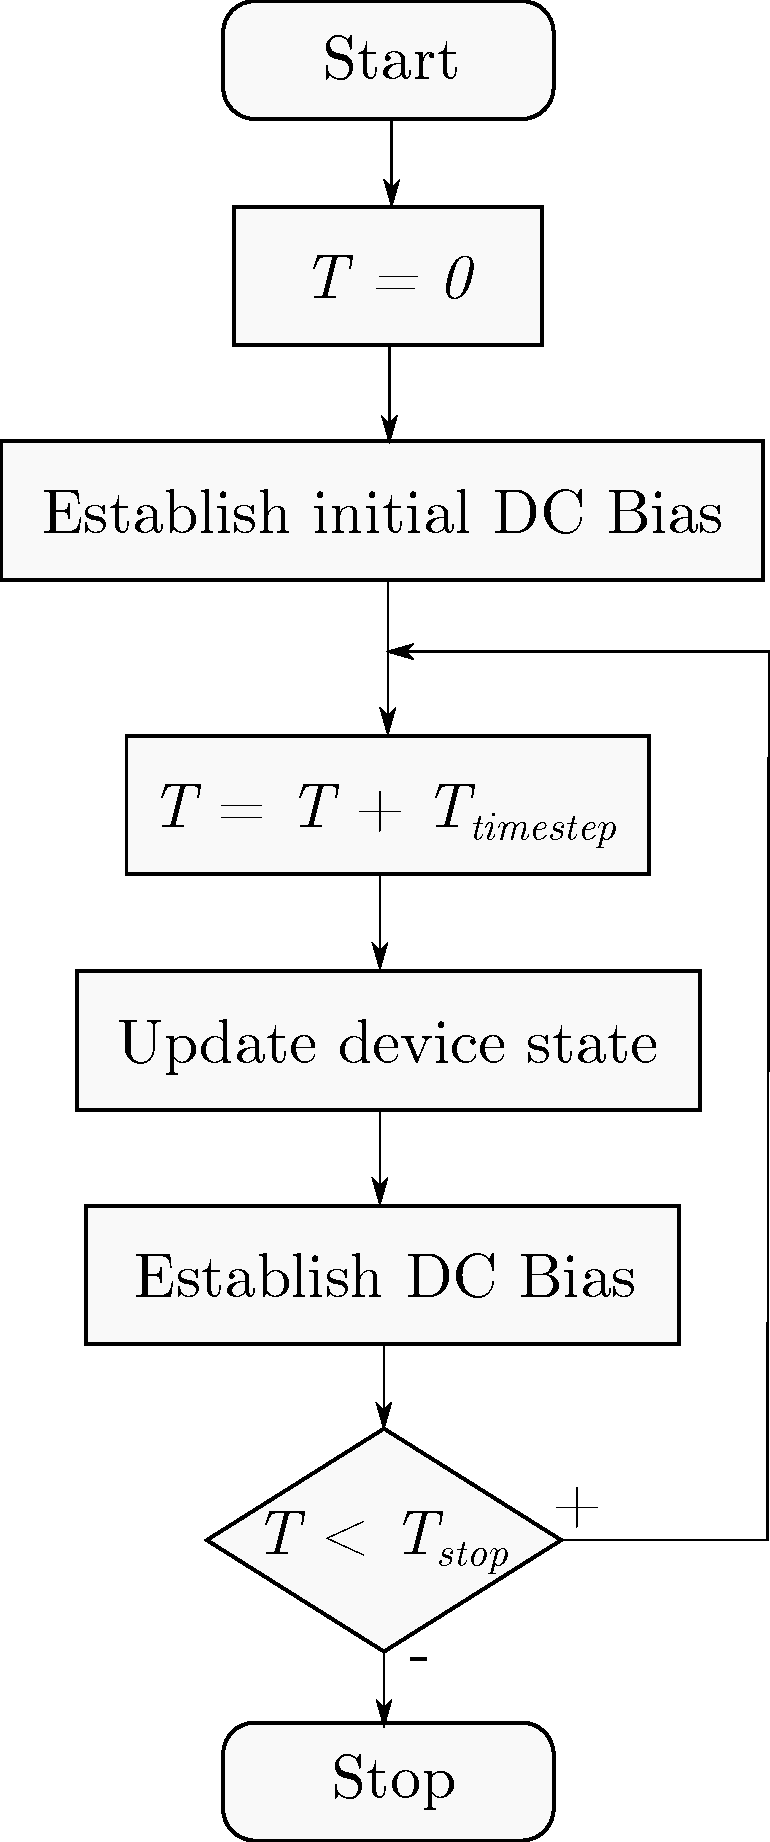
\includegraphics[width=.3\linewidth]{transient-analysis-diagram}
	\caption{Top level description of the transient analysis algorithm}
	\label{fig:analysis-transient-top-level}
\end{figure}

The simulation starts by calculating the initial DC bias of the circuit, during which capacitor and inductor devices are modeled as ideal open circuits and closed circuits, respectively. After the initial state of the circuit is established, the state of of active devices like capacitors and inductors, or nonconstant voltage and current sources is updated to reflect the time passed between the two successive timepoints. To reflect the energy stored in the capacitor and inductor devices, these devices are replaced by so called \textit{companion models}, which consist of either voltage or current source and a resistor. Parameters of the devices in the companion models are recomputed in each succesive timepoint (technical details will be explained later). Then a DC bias calculation is performed for the next timepoint and the process is repeated for the whole simulated period.

The details of DC bias calculation are described in the following subsections.
\subsubsection{DC Bias Calculation} 

We will demonstrate the DC bias calculation on the circuit shown in figure~\ref{fig:analysis:ls-bias-circuit}. Different colors of the devices will serve a purpose later.

\begin{figure}[h]
\begin{circuitdev}
	(0,0) 
	to[V=12<\volt>,invert,color=red] (3,0) node[circ,label={-90:$1$}]{}
	-- (6,0)
	to[R, l=5<\ohm>, ,color=blue] (6,3) node[circ,label={3:$3$}]{}
	to[R, l=5<\ohm>, color=green] (3,3) node[circ,label={$2$}]{}
	to[R, l=10<\ohm>, color=orange] (0,3)
	-- (0,0)
	
	(3,0) to[R, l=10<\ohm>,color=purple] (3,3)
	(0,1.5) -- (-0.5,1.5) node[ground]{}
\end{circuitdev}	
	\caption{Example circuit for DC bias calculation.}
	\label{fig:analysis:ls-bias-circuit}
\end{figure}


To calculate the node voltages and branch currents, the equations corresponding to the Kirchhoff's circuit laws must be formulated. There are several methods for algorithmic formulation of the circuit equations. As an example, we will show the \textit{Modified Nodal Analysis} (MNA) method. In MNA, there is a template for each device type's contribution to the equation system, which is called a device's \textit{stamp}. Device stamps for constant voltage source and resistor are shown in figure~\ref{fig:device-stamps}. An important thing to notice is that voltage sources (and some other devices) require an additional variable in the equation system for calculating the current flowing through the device.

\begin{figure}[h]
		\centering
		\begin{circuitdev}
			(0,0) node[label=N+]{} to[V, l=V, *-*, i_>=$I_V$] (3,0) node[label=N-]{}
			
			
			(9,0) node[label=N+]{} to[R, l=R, *-*] (12,0) node[label=N-]{}
		\end{circuitdev}
\[\begin{bmatrix}
	 &  & 1  \\
	 &  & -1 \\
	1 & -1 & 
\end{bmatrix} \cdot 
\begin{bmatrix}
V_{N+}\\
V_{N-}\\
I_V
\end{bmatrix}
=
\begin{bmatrix}
 \\
 \\
 V
\end{bmatrix}
\qquad
\qquad
\qquad
\begin{bmatrix}
	\frac{1}{R}& -\frac{1}{R}  \\
-\frac{1}{R}	& \frac{1}{R} \\
	\end{bmatrix}
\cdot
\begin{bmatrix}
V_{N+}\\
V_{N-}\\
\end{bmatrix}
=
\begin{bmatrix}
	\\
	\color{white}{f}
\end{bmatrix}\]
	\caption{Device stamps for the voltage source and resistor}
	\label{fig:device-stamps}
\end{figure}

Formulation of the circuit using MNA is done by iterating through the list of circuit devices and "stamping" them into the equation system. When applied to the circuit in figure~\ref{fig:analysis:ls-bias-circuit} MNA creates the following equation system shown in figure~\ref{fig:equation-example}. The contribution from each device is shown in the same color as the device.

\begin{figure}[h]
	\centering
	\[
	\color{black}
	\begin{bmatrix}
	\mathcolor{orange}{\frac{1}{10}}	&0	&	\mathcolor{orange}{-\frac{1}{10}}  	&0 	&0	& 0 \mathcolor{red}{-1}\\
	0	&	\mathcolor{purple}{\frac{1}{10}} + \mathcolor{blue}{\frac{1}{5}}	&	\mathcolor{purple}{-\frac{1}{10}}  	& \mathcolor{blue}{-\frac{1}{5}}	&0	&  \mathcolor{red}{1}\\
	\mathcolor{orange}{-\frac{1}{10}}	&	\mathcolor{purple}{-\frac{1}{10}}	&	\mathcolor{orange}{\frac{1}{10}} + \mathcolor{purple}{\frac{1}{10}} + \mathcolor{green}{\frac{1}{5}} 	&  \mathcolor{green}{-\frac{1}{5}} 	&0 & 0  \\
	0	&\mathcolor{blue}{-\frac{1}{5}}	& \mathcolor{green}{-\frac{1}{5}} 	& \mathcolor{blue}{\frac{1}{5}} + \mathcolor{green}{\frac{1}{5}} &0	&0 \\
	\mathcolor{red}{-1}	& \mathcolor{red}{1}	&0  	&0 	&0	&0
	\end{bmatrix} \cdot 
	\begin{bmatrix}
	V_0\\
	V_1\\
	V_2\\
	V_3\\
	\mathcolor{red}{I_V}
	\end{bmatrix}
	=
	\begin{bmatrix}
	0\\
	0\\
	0\\
	0\\
	\mathcolor{red}{12}
	\end{bmatrix}
	\]
	\caption{Equation system after stamping devices from our circuit}
	\label{fig:equation-example}
\end{figure}

Because node 0 corresponds to the ground node, it always holds that $V_0 = 0$. Therefore, the corresponding row and column can be eliminated. By solving the resulting equation system, we obtain the values $V_1 = 12$, $V_2=10$, $V_3=8$ and $I_V=-0.8$. Branch currents flowing through the resistors can be then trivially calculated using the formula $I_R = U_R/R$. 

\subsubsection{DC Bias Calculation - Nonlinear Devices}
In the preceding example, only \textit{linear} devices were used in the circuit. This means that the resulting equation system was also linear and an exact solution could be obtained. Another situation arises if a nonlinear device such as diode is used in the circuit. A semiconductor diode has nonlinear I-V characteristic which is approximated by the Shockley equation shown in figure~\ref{fig:diode-iv}.

\begin{figure}[h]
	\centering
	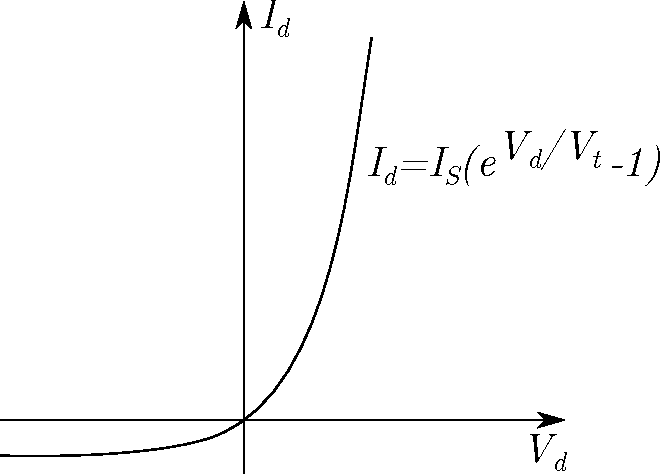
\includegraphics[width=0.32\linewidth]{diode-iv}
	\caption{I-V characteristic of a diode}
	\label{fig:diode-iv}
\end{figure}

Circuits containing such devices can no longer be characterized by a system of linear equations. Instead, a system of nonlinear equations needs to be solved. Such systems are solved iteratively by the Newton-Raphson method. In DC bias calculation, the Newton-Raphson algorithm is realized by repeatedly linearizing the I-V characteristics of nonlinear devices at the current candidate DC bias and solving the linearized equation system, to obtain the next candidate DC bias. Figure~\ref{fig:diode-equivalent} shows the linearization process on the diode example from figure~\ref{fig:diode-iv} around $V_B$, which is a current guess of the voltage across the diode. The linearized I-V characteristic then corresponds to replacing the diode by an \textit{equivalent circuit} consisting of a current source with $ I_{eq} $ current and a resistor with $ G_{eq} $ conductance, as shown in the figure.

\begin{figure}[h]
	\centering
		\begin{subfigure}{0.32\linewidth}
			\centering
			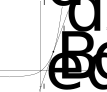
\includegraphics[width=\linewidth]{linearizing-diode}
		\end{subfigure}
		\begin{subfigure}{0.65\linewidth}
			\centering
			\begin{circuitdev}
				(-1.5,0) node[circ,label=1:+]{} to[D,i=$I_d$] (-1.5,-4) node[circ, label=1:-]{}
				
				(4,0) node[circ, label=1:+]{} -- (4,-0.5) -- (3,-0.5) to[I, a=$I_{eq}$] (3,-3.5) -- (4,-3.5) -- (4,-4) node[circ, label=1:-]{}
				
				(4,-0.5) -- (5,-0.5) to[R, l=$G_{eq}$] (5,-3.5) -- (4,-3.5);
				
					\draw [decoration={markings,mark=at position 1 with
					{\arrow[scale=3,>=stealth]{>}}},postaction={decorate}] (-0.5,-2) -- (1,-2)
			\end{circuitdev}
		\end{subfigure}
	\caption{Linear equivalent circuit for the diode}
	\label{fig:diode-equivalent}
\end{figure}

This iterative process stops when the difference between the diode currents in two consecutive solutions fits in the relative and absolute tolerances, which are parameters of the simulation. Another simulation parameter is the upper limit on the number of Newton-Raphson iterations. If the solution does not converge by the specified limit, then the simulation is aborted.

\subsubsection{DC Bias Calculation - Energy Storage Devices}

We have already briefly mentioned at the beginning of the subsection that capacitor and inductor devices are modeled by their companion models, which characterize the I-V characteristic of the device for the current timepoint. Figure~\ref{fig:capacitor-equivalent} shows the companion models for capacitor and inductor devices.

\begin{figure}[h]
	\centering
	\begin{subfigure}{0.49\linewidth}
		\centering
		\begin{circuitdev}
			(-0.5,0) node[circ,label=1:+]{} to[C] (-0.5,-4) node[circ, label=1:-]{}
			
			(4,0) node[circ, label=1:+]{} -- (4,-0.5) -- (3,-0.5) to[I] (3,-3.5) -- (4,-3.5) -- (4,-4) node[circ, label=1:-]{}
			
			(4,-0.5) -- (5,-0.5) to[R] (5,-3.5) -- (4,-3.5);
			\draw [decoration={markings,mark=at position 1 with
				{\arrow[scale=3,>=stealth]{>}}},postaction={decorate}] (0.5,-2) -- (2,-2)
		\end{circuitdev}
		\subcaption{Capacitor}
	\end{subfigure}\begin{subfigure}{0.49\linewidth}
			\centering
		\begin{circuitdev}
			[white] (0.5,0)  to[V,color=white] (0.5,-4); \draw
			
			(0.5,0) node[circ,label=1:+]{} to[L] (0.5,-4) node[circ, label=1:-]{}
			
			(4,0) node[circ, label=1:+]{} to[R] (4,-2) to[V, invert] (4,-4) node[circ, label=1:-]{};
			
			\draw [decoration={markings,mark=at position 1 with
				{\arrow[scale=3,>=stealth]{>}}},postaction={decorate}] (1.5,-2) -- (3,-2)
		\end{circuitdev}
		\subcaption{Inductor}
	\end{subfigure}
	\caption{Companion models of capacitor and inductor}
	\label{fig:capacitor-equivalent}
\end{figure}

Parameters of the companion models are updated each timepoint via \textit{numerical integration} to reflect the energy stored in the device. However, if the timestep used in the simulation is too big, local errors made during the integration may accumulate and therefore produce unrealistic results of the simulation. On the other hand, smaller timestep means that the simulation will take longer. Modern simulators internally choose the timestep dynamically: small timestep values when the values of companion models change rapidly, and greater timestep values otherwise. This way the simulator preserves both speed and accuracy. This process is illustrated in figure~\ref{fig:dynamic-timestep}.

\begin{figure}[h]
	\centering
	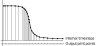
\includegraphics[width=.8\linewidth]{dynamic-timestep}
	\caption{Depiction of dynamic timestep mechanism, reproduced from Inside SPICE \cite{inside_spice}}
	\label{fig:dynamic-timestep}
\end{figure}

This process is realized by iterating individual devices and estimating the maximum timestep for which the truncation error does not exceed the simulator tolerances. The minimum of these values is then chosen as the next timestep. 

To implement transient analysis as described so far, we need to make important decisions regarding individual parts of the algorithm. The main parts that need to be analyzed are the method used for equation system formulation, representation of the equation system, choice of numerical integration method, choice of timestep control mechanism and the interface that will be required from device logic implementations.

\subsection{Choice of Equation System Formulation}

As we mentioned in the previous subsection, there are several methods for automated creation of the circuit equation system. Many of those are described in great depth in Nagel's PhD thesis \cite{Nagel:M520}, chapter III. 

Nagel includes a comparison of the methods with respect to the size of the equation and the programmatic effort of implementing these methods. His research shows that the MNA method which was used in the example in section~\ref{chap:analysis:transient-overview} produces comparatively smaller equation systems than other methods. 

Another advantage of using the MNA method is that it does not require finding loops and trees in the circuit graph, which are required by methods like Modified Tableau Analysis. Instead, as we have shown earlier, all devices contribute to the equation system via a device type stamp. Also, adding a new device type does not require changes to the formulation method, because the device stamp can be made part of the device's implementation.

For the reasons above, we decided to use the MNA method during transient analysis.

\subsection{Equation System Abstraction}
\label{chap:analysis:equation}
There are multiple ways of representing the equation system. The most straightforward way is representing the equation matrix as a full two-dimensional array. Such a representation is intuitive and easy to manipulate in the program. However, if the equation matrix is sparse (many coefficients are equal to 0), this representation is inefficient. When using MNA, the number of nonzero elements in a row is roughly proportional to the number of devices that connect to that node. This means that in large circuits, where only a small number of devices connects to the same node at once, it would be more appropriate to use a sparse matrix representation.

We decided to use the full 2D array representation for simplicity, but in case that this representation would prove to be an issue in the future, we would like to change the implementation without affecting the user code. Therefore, we have to expose the equation system under an interface that can be efficiently implemented by sparse matrix representations too.

There is also an additional requirement on the equation system implementation. As we have shown in figure~\ref{fig:device-stamps}, devices may need an additional circuit variable to be correctly simulated. The equation system implementation therefore needs to support adding additional variables at least during the initialization phase of the simulation.

Because we decided to use the MNA method for equation system formulation, each device needs to modify only a small fixed set of equation system coefficients corresponding to the device's stamp. We have therefore decided to use the interface illustrated in figure~\ref{fig:analysis-equationsystem}. During the initialization phase of the simulation, each device would request any number of additional variables that it requires, and specify which equation system coefficients it contributes to. Access to these coefficients will be then provided using a proxy object for each accessed coefficient. 

\begin{figure}[h]
	\centering
	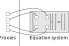
\includegraphics[width=0.4\linewidth]{analysis-equationsystem}
	\caption{Equation system abstraction}
	\label{fig:analysis-equationsystem}
\end{figure}

This interface is general enough to allow any internal equation system representation while providing efficient access to individual coefficients.

\subsection{Choice of Numerical Integration Method}
In the description of transient analysis of energy storage devices, we mentioned that the inner state of the device is updated based on the circuit state of the previous timepoint using numerical integration. Commonly used integration methods include Backward Euler, Trapezoidal Rule, and Gear method. A summary of these and other numerical integration methods can be found in QUCS Technical Papers, section 6.1. Nagel's PhD thesis also provides a detailed analysis of common numerical integration methods in chapter VI. None of these methods can be considered best for circuit simulation. For example, although the trapezoidal rule is very good in terms of accuracy and speed, it may sometimes lead to a phenomenon called \textit{trapezoidal ringing}, which means that the value oscilates around the exact value. The trapezoidal ringing is shown in figure~\ref{fig:trap-ringing}.

\begin{figure}[h]
	\centering
	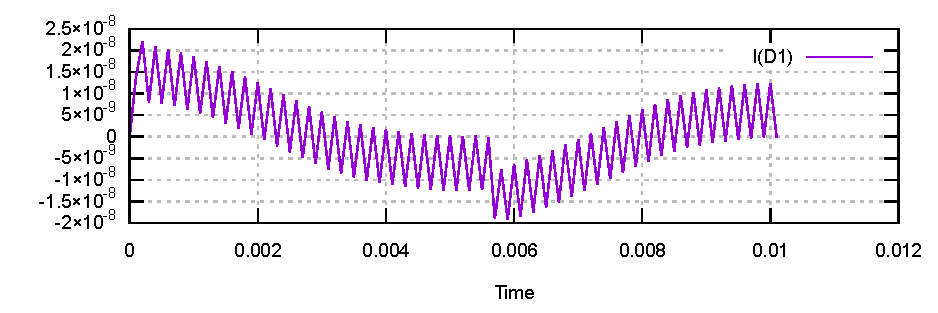
\includegraphics[width=0.8\linewidth]{04-fig-back-to-back-trap}
	\caption{Trapezoidal ringing.}
	\label{fig:trap-ringing}
\end{figure}

For this reason, modern circuit simulators implement multiple integration methods. If the default method proves inappropriate, the user can instruct the simulator to use a different method. We would therefore like to allow using different integration methods in our simulator, and even allow the user to add new integration methods.
%As a proof of concept, we will implement Backward Euler, Trapezoidal Rule and Gear integration methods. \todo{remove the last sentence?}

\subsection{Choice of Timestep}
\label{chap:analysis-timestep}
While describing the simulation of energy storage devices back in section~\ref{chap:analysis:transient-overview}, we briefly mentioned that additional precision can be achieved by choosing the timestep dynamically. The dynamic methods choose the timestep such that the error introduced by the integration method is less than a certain threshold. The timestep choice therefore depends on the integration method and the device's state in previous timepoints.

We decided to simplify the library's implementation and not implement the dynamic timestep in the initial version of the library. Therefore, the library will rely on the user to specify an appropriate timestep value that will be used throughout the simulation. However, the dynamic timestep is an attractive feature and we would like to add it in the next versions of the library.
